% !TEX root = main.tex

\section{Temporal deployment changes}\label{sec:longitudinal}
\rhtodo{Is this still going to stay in? It's too much work to complete. Although if Fig 9 is complete and the numbers are robust, it could be worth saying that overall, what we see is stable. Then again, the methodology of Censys is different, and I am not sure of their coverage of anycast prefixes, they scan from other VPs, etc. Too much for now?} % G: removed censys stuff. If we need space, let's just add a paragraph about it like ralph suggested.
%In this section, we longitudinally investigate changes in anycasted services in stable anycast prefixes (long-term prefixes) as well as fluctuations (short-lived prefixes).

\iffalse
\subsection{Long-term}
First, we make use of monthly \laces and \gls{cuids}
to observe long-term trends in anycast.

We use \gls{cuids} as it provides historical data
with which we can compare from the start of \laces data in February 2024.
This analysis provides a 2~year analysis.
First, we look at deployment changes visible in anycast. % TODO

Now, we look at changes in services offered. % TODO
% RH: previous data (Oct 2024) showed 150k QUIC ports -> why did it decrease? something to look at for longitudinal analysis
\fi

%\subsection{Short-term}
Prior work has showed that anycast deployments can exhibit volatility, with certain prefixes being advertised as anycast in short-time periods~\cite{Hendriks_LACeS_An_Open_2025}.
To better understand these dynamics, we analyze the services hosted on short-lived anycast prefixes over a 14-day longitudinal measurement from our European \gls{vp}.
As shown in \cref{fig:services_longitudinal}, the most widely deployed services are also those most frequently impacted by daily prefix advertisement and withdrawal events.
Over the measurement period, 545 unique anycast prefixes transition in or out, averaging 109 daily fluctuations (with a standard deviation of 18).
The services most affected by this churn are HTTP, DNS, and SSH.
These fluctuations may stem from automated routing changes triggered by service availability monitoring--a practice for services like DNS~\cite{Abley_SoftwareApproachDistributing_2004}.
Withdrawing an anycast prefix due to the failure of a single service can inadvertently render all other services advertised on that same prefix unavailable~\cite{rfc4786}.
However, the service could be advertised in another location, and hence validating its availability would require a qualitative survey.
Notably, we find that 77\% of the prefixes experiencing this volatility belong to small-scale deployments operating with only two \glspl{pop}.
% see rfc4786 section 4.4.1
%However, rapid advertisement or withdrawal fluctuations can cause problems increase of CPU load on servers or unavailability of the service~\cite{rfc4786}.
% see rfc4786 section 4.4.4; but checking rfc2439 sec. 2, route flapping is attributed to very fast BGP announcements (hours), which our data don't cover.

\begin{figure}[tb]
\centering
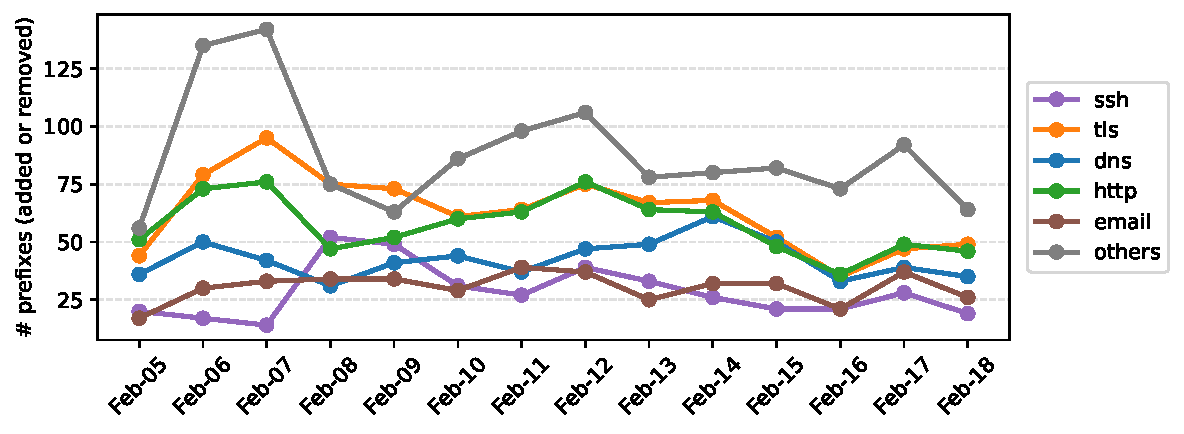
\includegraphics[width=\columnwidth]{./data/plots/services_longitudinal}
\caption{Longitudinal view on services added to and removed from anycast prefixes.}
\label{fig:services_longitudinal}
\end{figure}
